\documentclass[a4paper]{article} 
\addtolength{\hoffset}{-2.25cm}
\addtolength{\textwidth}{4.5cm}
\addtolength{\voffset}{-3.25cm}
\addtolength{\textheight}{5cm}
\setlength{\parskip}{0pt}
\setlength{\parindent}{0in}

\usepackage[square,sort,comma,numbers]{natbib}
\usepackage{blindtext} % Package to generate dummy text
\usepackage{charter} % Use the Charter font
\usepackage[utf8]{inputenc} % Use UTF-8 encoding
\usepackage{microtype} % Slightly tweak font spacing for aesthetics
\usepackage{amsthm, amsmath, amssymb} % Mathematical typesetting
\usepackage{float} % Improved interface for floating objects
\usepackage{hyperref} % For hyperlinks in the PDF
\usepackage{graphicx, multicol} % Enhanced support for graphics
\usepackage{xcolor} % Driver-independent color extensions
\usepackage{pseudocode} % Environment for specifying algorithms in a natural way
\usepackage[mmddyy]{datetime} % Uses YEAR-MONTH-DAY format for dates

\usepackage{fancyhdr} % Headers and footers
\pagestyle{fancy} % All pages have headers and footers
\fancyhead{}\renewcommand{\headrulewidth}{0pt} % Blank out the default header
\fancyfoot[L]{} % Custom footer text
\fancyfoot[C]{} % Custom footer text
\fancyfoot[R]{\thepage} % Custom footer text
\newcommand{\note}[1]{\marginpar{\scriptsize \textcolor{red}{#1}}} % Enables comments in red on margin

\DeclareMathOperator*{\argmin}{arg\,min}

%----------------------------------------------------------------------------------------

\newcommand{\yourname}{Balthazar Neveu}
\newcommand{\youremail}{balthazarneveu@gmail.com}
\newcommand{\assignmentnumber}{2}

\begin{document}

\fancyhead[C]{}
\hrule \medskip
\begin{minipage}{0.295\textwidth} 
\raggedright
\footnotesize
\yourname \hfill\\
\youremail
\end{minipage}
\begin{minipage}{0.4\textwidth} 
\centering 
\large 
Lab session \# \assignmentnumber\\ 
\normalsize 
ALTEGRAD 2023\\ 
\end{minipage}
\begin{minipage}{0.295\textwidth} 
\raggedleft
\today\hfill\\
\end{minipage}
\medskip\hrule 
\bigskip



\part[short]{Analyzing a Real-World Graph}

\section*{Coding results}

\subsection*{Task 1 : Basic graph statistics extraction}
\begin{verbatim}
{'total_edges': 25998,
 'total_nodes': 9877}
max number of edges 48772626
\end{verbatim}


\subsection*{Task 2 : Extract the connected components of the graph}
\begin{verbatim}
Graph has 429 connected components
Largest connected component:
{'total_edges': 24827,
 'total_nodes': 8638}
8638 total_nodes represent 87.46% of the graph
24827 total_edges represent 95.50% of the graph
\end{verbatim}


\subsection*{Task 3 : Statistics on the degrees of the nodes of the graph}
\begin{verbatim}
{'degree_of_nodes': {'max': 65,
                     'mean': 5.264351523742027,
                     'median': 3.0,
                     'min': 1}}
\end{verbatim}


\subsection*{Task 4 : Degree histogram plot}
\begin{verbatim}
\end{verbatim}\begin{figure}[ht]
        \centering
        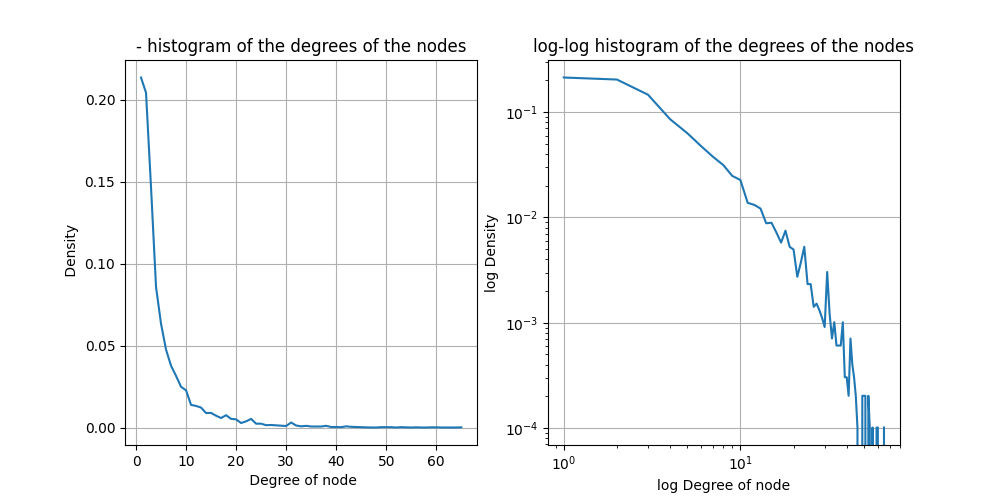
\includegraphics[width=.6\textwidth]{figures/histogram_degree_of_nodes.png}
        \caption{Histogram of degrees of the nodes}
\end{figure}
\begin{verbatim}
\end{verbatim}


\subsection*{Task 5 : Global clustering coefficient}
\begin{verbatim}
Graph clustering coefficient: 0.284
\end{verbatim}


\section{Question 1:}
Assume $G = (V, E)$ is an undirected graph of n nodes without self-loops. $|V|=n$.
\subsection*{Number of edges}
The maximum number of edges is the cardinal of the set of possible combinations of 2 nodes chosen from n nodes.
which is equal to the binomial coefficient $\binom{n}{2} = \frac{n!}{2! (n-2)!}$
\begin{equation}\label{eq 1.1}
|E| \leq \frac{n*(n-1)}{2}
\end{equation}
This can also be viewed when writing the adjacency matrix of a complete graph.
\begin{itemize}
    \item  A matrix full of 1 has $n^2$ elements
    \item set the diagonal to 0 to remove the self loops. $n*(n-1)$ elements
    \item Divide by two since we consider an undirected graph.
\end{itemize}


In the code the property is verified through an assert.

\subsection*{Number of triangles}
The maximum number of triangles is $\binom{n}{3} = \frac{n!}{3! * (n-3)!} = \frac{n*(n-1)(n-2)}{6}$ 
when choosing the combination of 3 nodes from n nodes.


\section{Question 2 : 2 graphs having the same degree distribution $\not \implies$ isomorphic}

If two graphs have the same degree distribution, it does not imply that they are isomorphic to each other.
The simplest counter-example with degrees of nodes of 2 is presented 
in \ref{fig:graph_triangle_vs_three_single_loops},
it's a bit of a degenerate case as we're using the fact that a loop adds two to the degree in case of undirected graphs.
Below are four cases illustrating the counter example.
\ref{fig:graph_compare_triangle_hexagon} shows an hexagon versus 2 triangles 
which is the most pleasant example to visualize.



\begin{figure}[ht]
    \centering
    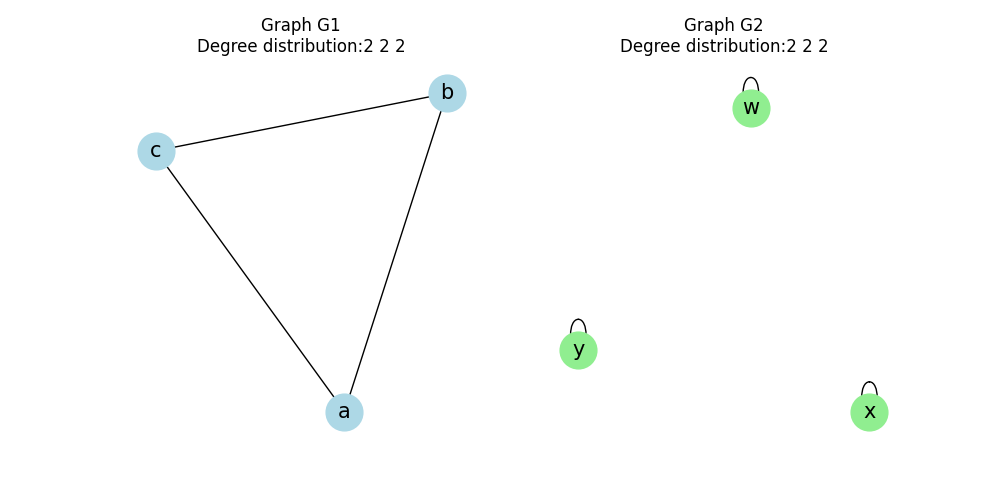
\includegraphics[width=.6\textwidth]{figures/graph_triangle_vs_three_single_loops.png}
    \caption{Graphs G1 is a triangle and G2 is made of 3 isolated nodes with a self loop.They have the same degree distribution (every node has a degree of 2)but are not isomorphic to each other.}
    \label{fig:graph_triangle_vs_three_single_loops}
\end{figure}



\begin{figure}[ht]
    \centering
    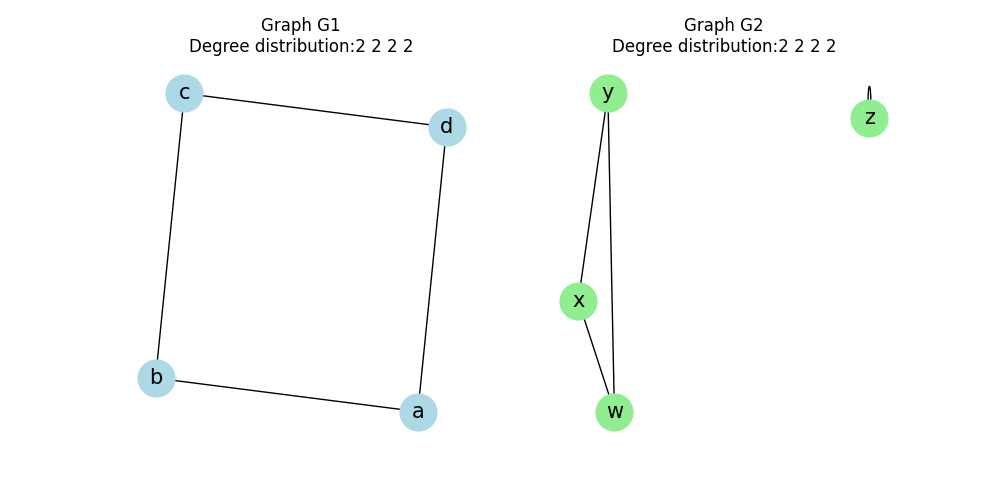
\includegraphics[width=.6\textwidth]{figures/graph_rect_vs_triangle_plus_single_loop.png}
    \caption{G1 is a rectangle, G2 is made of a triangle and a single node with a self loop.}
    \label{fig:graph_rect_vs_triangle_plus_single_loop}
\end{figure}



\begin{figure}[ht]
    \centering
    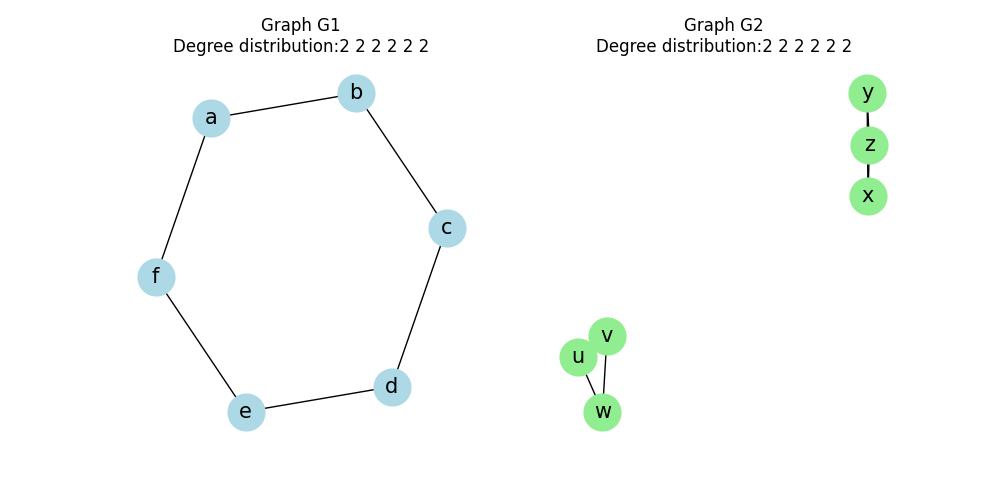
\includegraphics[width=.6\textwidth]{figures/graph_compare_triangle_hexagon.png}
    \caption{G1 is an hexagon, it has 6 edges. G2 has 2 separate triangles.All nodes have a degree of 2, G1 and G2 have the same degree histograms.But they are not isomorphic to each other}
    \label{fig:graph_compare_triangle_hexagon}
\end{figure}


\begin{figure}[ht]
    \centering
    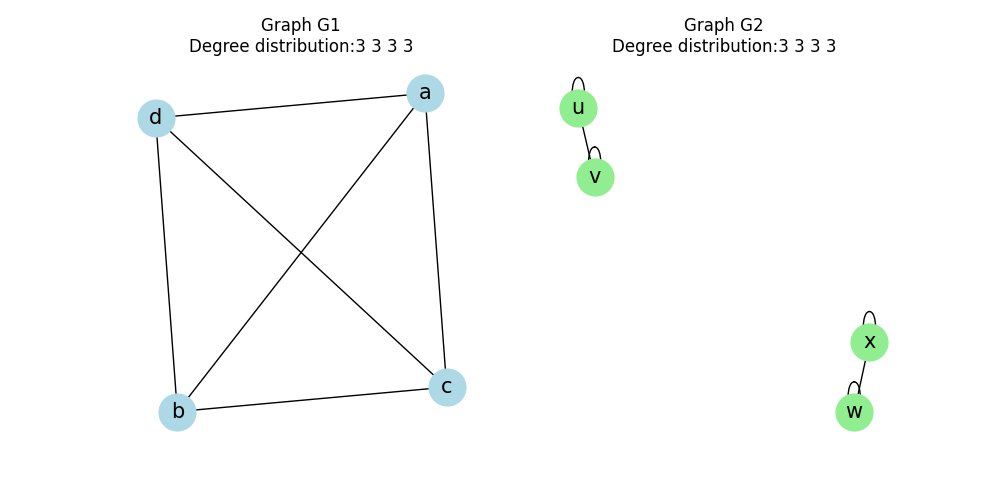
\includegraphics[width=.6\textwidth]{figures/graph_compare_quad.png}
    \caption{Counter example where all nodes have a degree of 3.G1=(a-b, b-c, c-a, b-d, d-c, d-a) is a rectangle with its diagonalsG2=(u-v, u-u, v-v, w-x, w-w, x-x) are 2 segment where the end nodes have self loops}
    \label{fig:graph_compare_quad}
\end{figure}

\pagebreak
\subsection*{Question 3 : n-cycle graphs}
\begin{itemize}
    \item Clustering coefficient of the triangle $C_3$ is $1=\frac{1}{1+0}$
    \item Clustering coefficient of cycle graphs $C_n$ where $n \geq 4$ is $0=\frac{0}{0+n}$
    as there are no closed triplets but only ($n$) open triplets. 
\end{itemize}
\begin{figure}[ht]
        \centering
        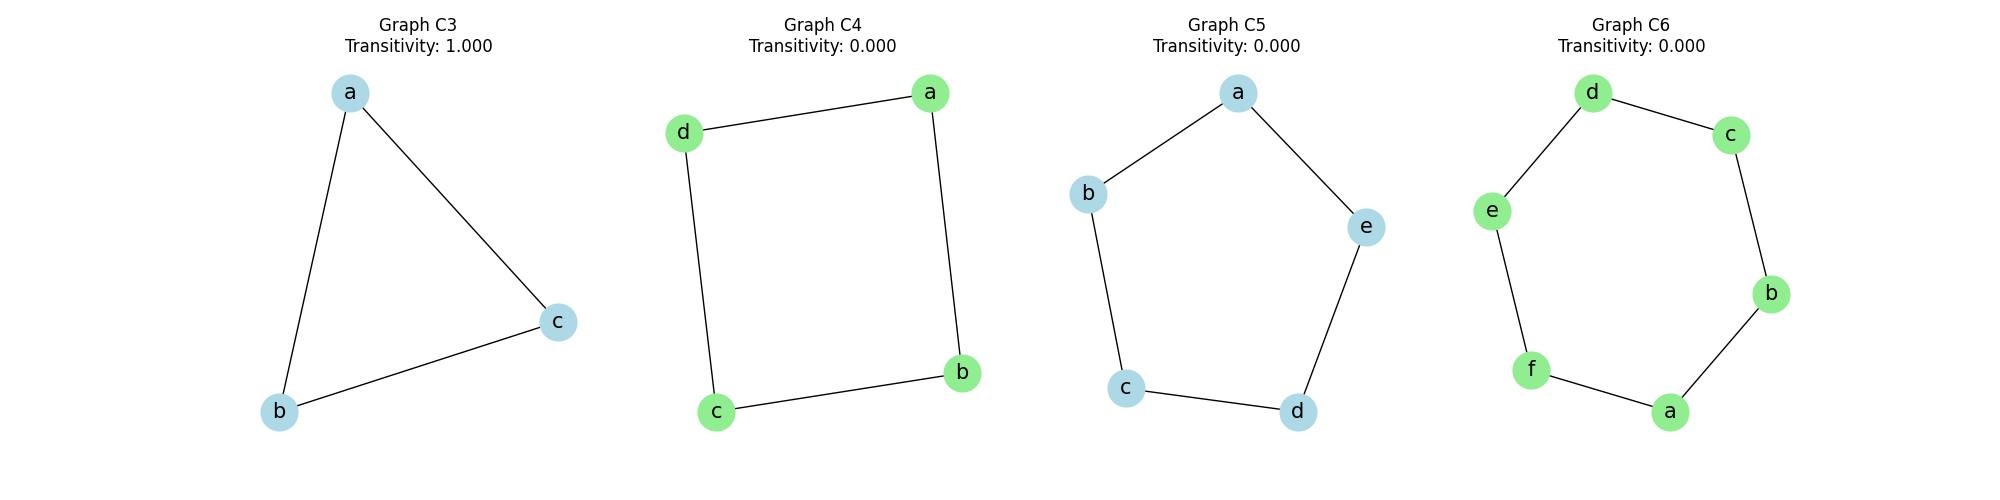
\includegraphics[width=.6\textwidth]{figures/cycle_graphs.png}
        \caption{Transitivity of $C_n$ cycle graphs becomes 0 if $n \geq 4$}
        \label{fig:cycle_graphs}
\end{figure}

\pagebreak
\part[short]{Community detection}

\pagebreak
\part[short]{Graph classification}

\subsection*{Task 10 : Cycle and graph dataset creation}

\begin{figure}[ht]
        \centering
        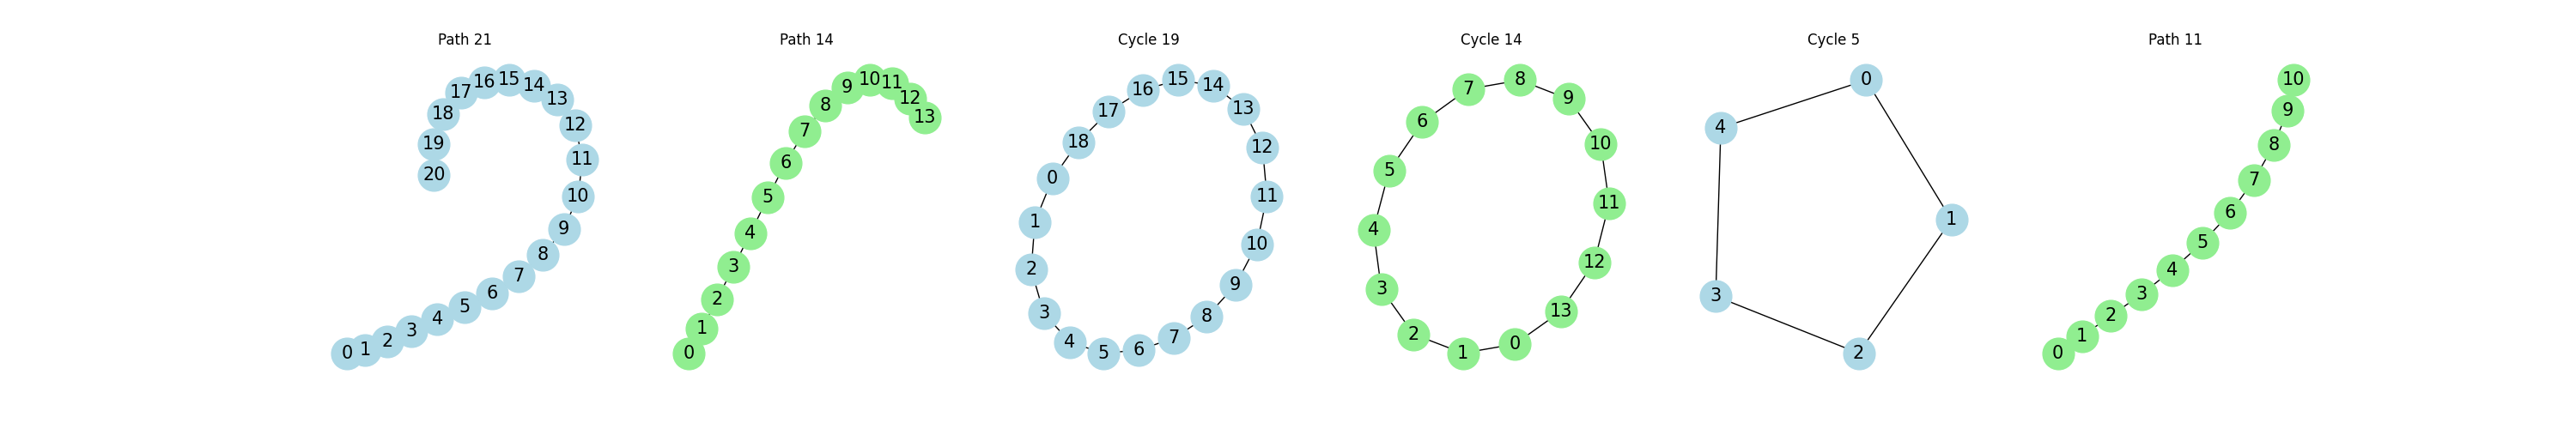
\includegraphics[width=1.\textwidth]{figures/cycle_and_paths_dataset.png}
        \caption{Dataset is made of cycles $C_n$ and paths $P_n$}
        \label{fig:cycle_and_paths_dataset}
\end{figure}


\section{Question 6 : Shortest path kernel}
In \ref{fig:P4_shortest_paths_computation} and \ref{fig:S4_shortest_paths_computation}, we show 
how we progressively build the shortest paths graph for the path $P_4$ and the start $S_4$.
Then we simply compute the distribution of the edges weights (=length) to get the so called "feature map" $\phi$.
We get:
\begin{itemize}
    \item $\phi(P_4)=[3, 2, 1, 0 ...]^T$
    \item $\phi(S_4)=[3, 3, 0, 0 ...]^T$
    \item $k(P_4, P_4) = 3^2 + 2^2 + 1^2 = 14$
    \item $k(P_4, S_4) = K(S_4, P_4) = 3*3+2*3+1*0 = 15$
    \item $k(S_4, S_4) = 3^2 + 3^2 = 18$
\end{itemize}

\begin{figure}[ht]
        \centering
        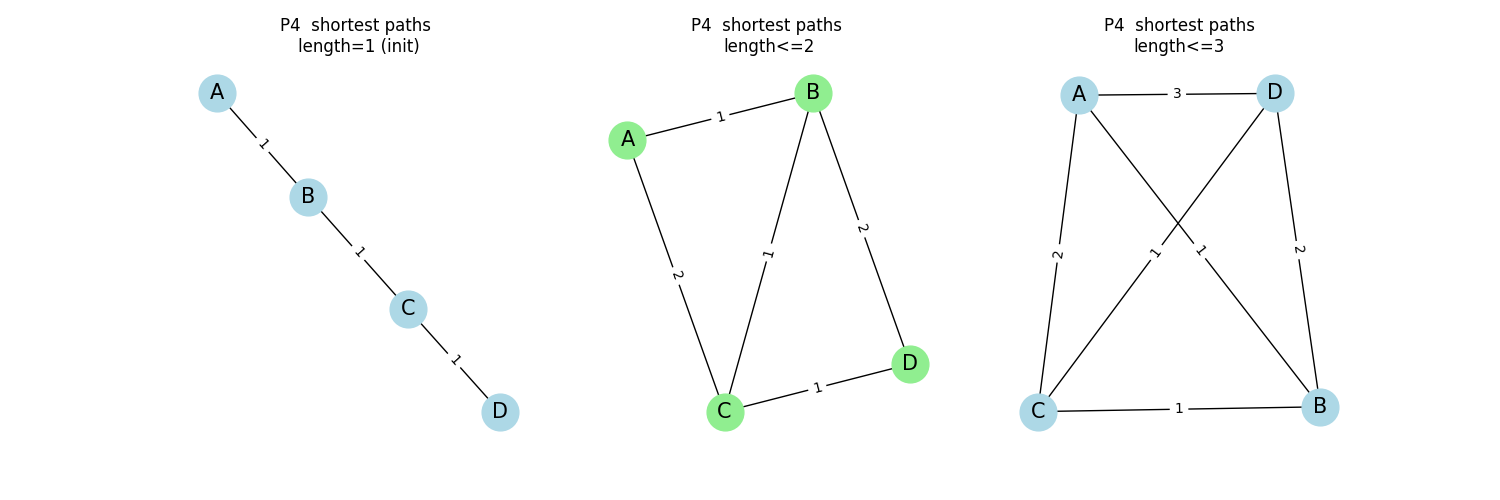
\includegraphics[width=1.\textwidth]{figures/P4_shortest_paths_computation.png}
        \caption{Path graph $P_4$, $\phi(P_4)=[3, 2, 1, 0 ...]^T$}
        \label{fig:P4_shortest_paths_computation}
\end{figure}

\begin{figure}[ht]
    \centering
    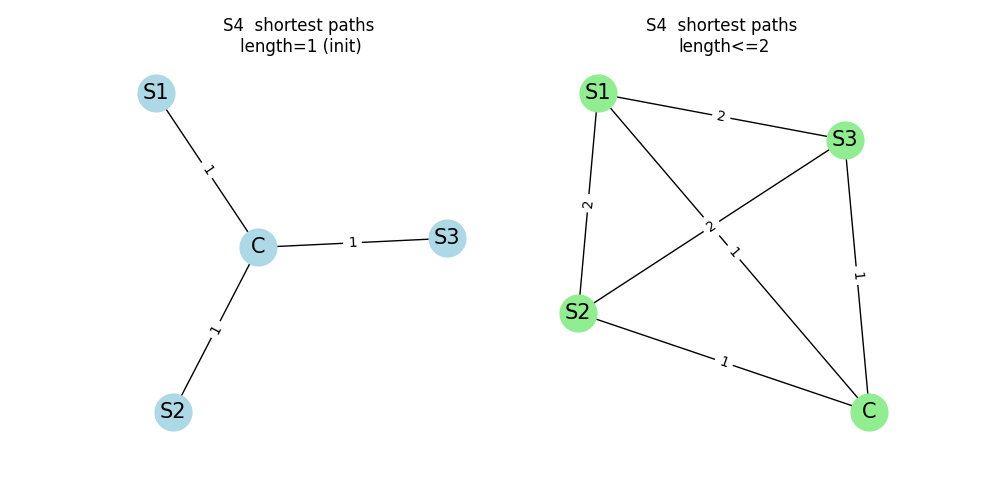
\includegraphics[width=.6\textwidth]{figures/S4_shortest_paths_computation.png}
    \caption{Start graph $S_4$ , $\phi(S_4)=[3, 3, 0, 0 ...]^T$}
    \label{fig:S4_shortest_paths_computation}
\end{figure}

\pagebreak
\section*{Task 11: Finding isomorphic graphlets in subgraphs}
We show in \ref{fig:finding_isomorphic_graphlets_subgraphs} and \ref{fig:finding_isomorphic_graphlets_subgraphs_triangle}
how to compute the feature maps for each sampled triplet subgraph.
We repeat this sampling process $N=200$ times for each graph.
\begin{figure}[ht]
    \centering
    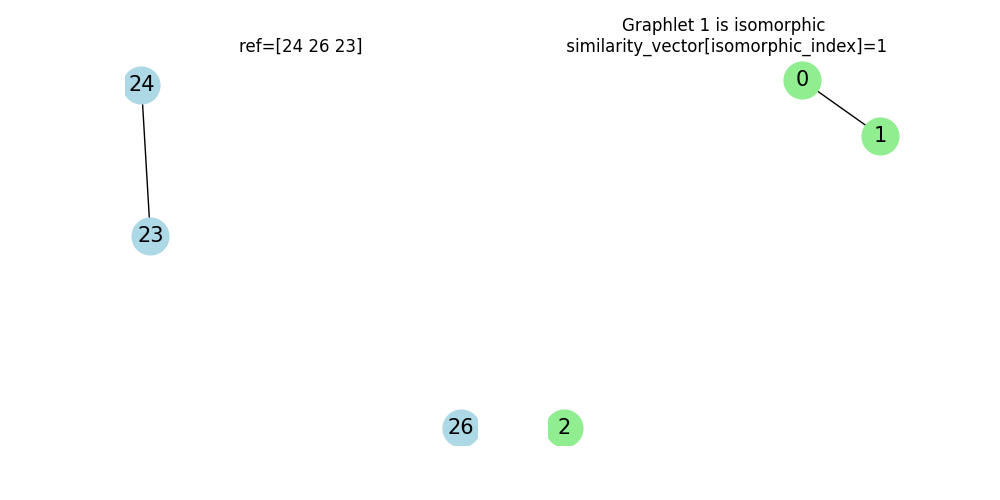
\includegraphics[width=.6\textwidth]{figures/finding_isomorphic_graphlets_subgraphs.png}
    \caption{Finding graphlet "$G_1$" (notation of the code) which is isomorphic with a randomly sampled subgraph made of 3 nodes.
    Feature vector is $[0, 1, 0, 0]^T$ for this subgraph}
    \label{fig:finding_isomorphic_graphlets_subgraphs}
\end{figure}

\begin{figure}[ht]
    \centering
    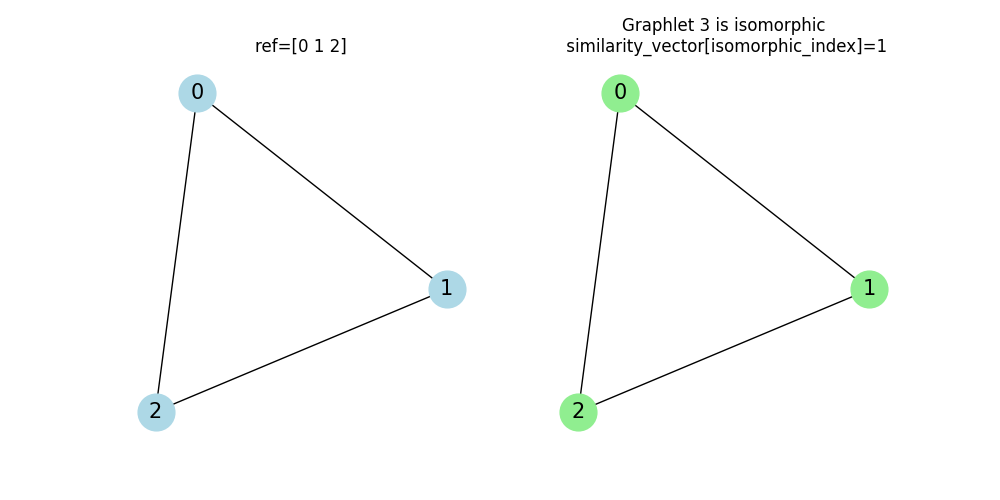
\includegraphics[width=.6\textwidth]{figures/finding_isomorphic_graphlets_subgraphs_triangle.png}
    \caption{Finding triangle graphlet "$G_3$" ( notation of the code) which is isomorphic with a randomly sampled subgraph made of 3 nodes?
    Feature vector is $[0, 0, 0, 1]^T$ for this subgraph}
    \label{fig:finding_isomorphic_graphlets_subgraphs_triangle}
\end{figure}
\pagebreak
%------------------------------------------------

\bibliographystyle{plain}
\bibliography{references}
\end{document}